\chapter{実験2}
\section{動機}
実験1で機械学習がうまくいかなかった原因には,
データ数が85と少なすぎたことが考えられた.

そこで,2回目のクラウドソーシングを行い
データ数を増やしたうえで,
LOOCV法を用いて実験を再度行うこととした.
\section{データセット}
実験1と同じ,\ref{sec:ch2:dataset}で抽出した
1076件のデータを用いた.
\section{クラウドソーシングの実施}
データ数を増やすため,実験1でクラウドソーシングの
対象としなかった画像を対象に,クラウドソーシングを
実験1とほぼ同様に行った.
\subsection{タスクインストラクション}
タスクインストラクションは実験1と同様に設定した.
\subsection{人数・値段・工夫した点}
データ数を増やすことを目的とするため,
1タスク当たりのワーカー数を1人と変更し,
以下のように,人数・値段を設定した.
\begin{itemize}
  \item 1タスク1ワーカー
  \item 1タスク当たりのワーカー報酬は\$0.02
  \item 1タスク当たりのAMT手数料は\$0.01
  \item 255タスク実施
\end{itemize}
よって
請求金額は,
255タスク$\times$1ワーカー$\times$\$0.03$=$\$7.65となった.
タスク数255は1000円という予算を考慮して決定した数である.
1タスク当たりの報酬額は実験1と同様であり,
アメリカの時給水準を十分に満足するものである.

\ref{sec:ch2:dataset}で抽出したデータの内,
実験1で対象としなかったものの中から
顔検出スコアが高い255件を抽出し,
筑波大学全学計算機システムWeb公開サービスを用いて埋め込んだ.
\section{クラウドソーシングの結果}
AMTでクラウドソーシングを行い,
255タスク$\times$1ワーカー$=255$件のデータを得た.
\subsection{ワーカー当たり回答数の分布}
\begin{figure}[tb]
\centering
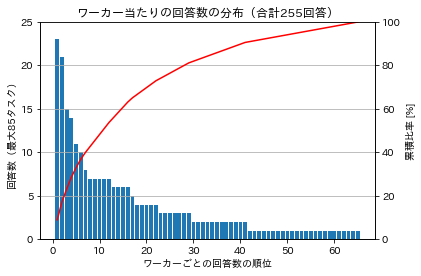
\includegraphics[width=10cm]{ch3/worker.png}
\caption{ワーカー当たりの回答数の分布(パレート図)
\label{fig:ch3:worker}}
\end{figure}
クラウドソーシングには65人のワーカーが
参加した.
ワーカー当たりの回答数の分布をパレート図にしたものを
図\ref{fig:ch3:worker}に示す.
これを見ると,1/6のワーカーが,
全体の50\%を回答していることがわかる.

実験1と同様に,
AMTでは,1ワーカー当たりが回答できるタスク上限数を
設定することができないため,このように,
一部のワーカーが多くを回答することがある.
\subsection{ラベルごとの分布}
実験2でのクラウドソーシングは,
1タスク当たり1ワーカーであるから,
多数決などを行わずに,ラベルの分布を得ることができる.

\begin{figure}[tb]
  \centering
  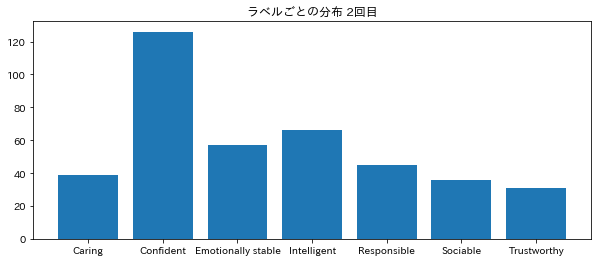
\includegraphics[width=10cm]{ch3/plot_label_2.png}
  \caption{2回目のクラウドソージングでのラベル数の分布
  \label{fig:ch3:label2}}
\end{figure}

2回目のクラウドソージングでのラベル数の分布を
プロットしたものを図\ref{fig:ch3:label2}に示す.
実験1の和集合データにおける分布である
図\ref{fig:ch2:svs}と比較すると,
ラベル数が多いラベルや少ないラベルが
ある程度共通していることがわかる.
\subsection{クラウドソーシング結果の連結}
実験2の目的はデータ数を増やしたうえで,
実験1を再度行うことであった.

そこで,実験1の85枚の画像に関するデータと
実験2の255枚の画像に関するデータを連結し,
計340枚のデータとすることにした.

ただし,実験1は1タスク当たり3ワーカー,
実験2は1タスク当たり1ワーカーのデータとなっており,
これらを連結することは単純には行えない
\footnote{タスク当たりのワーカー数が異なるデータを
連結することは決して研究手法として
お行儀が良いものでもないと思われるが,
今回はシステムを作ることが目的であるので,
妥協することにした.}.

そこで,実験1の単純多数決データと,
実験2のデータを連結することで,
実験2で用いるデータセットを作成した
\footnote{
実験が終わった後に気づいたが,
この連結手法は,実験1の単純多数決データと実験2のデータでは
画像当たりの平均ラベル数が有意に異なるため適切ではなかった.
適切な連結を行うには,実験1における3ワーカーのうち,
ランダムにワーカーを1人選択し,その回答を抽出したものに,
実験2の結果を統合すべきであったかもしれない.
}.
このデータのラベル数の分布を図\ref{fig:ch3:label_uni}
に示す.
\begin{figure}[tb]
  \centering
  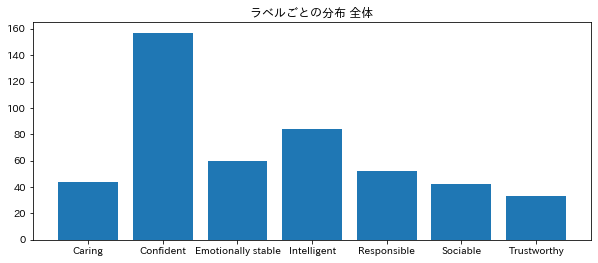
\includegraphics[width=10cm]{ch3/plot_label_uni.png}
  \caption{連結したデータでのラベル数の分布
  \label{fig:ch3:label_uni}}
\end{figure}
実験2ではこの連結したデータを利用して,
機械学習を行った.

\section{機械学習の実施}
実験1と異なる点として,k分割交差検定法ではなく,
Leave One Out Cross Validation(LOOCV法)を用いた.
LOOCV法は計算コストは高くなるものの,
正確な結果が期待できる.

他はすべて実験1と同じとした.
\section{機械学習の結果}

